\chapter{Back Propagation and Initialization}
\section{Review}

\begin{itemize}
\item
Neural-net and formulation; (section~\ref{sec:1:3})
\item
Training difficulty; (section~\ref{sec:1:4})
\begin{example}
Consider the multi-layer $(L=7)$ linear neural network with scalar input. The function shape of the loss function $y(w)\triangleq (w^7-1)^2$ is presented in Figure~(\ref{Fig:2:1})
\begin{figure}[H]
\centering
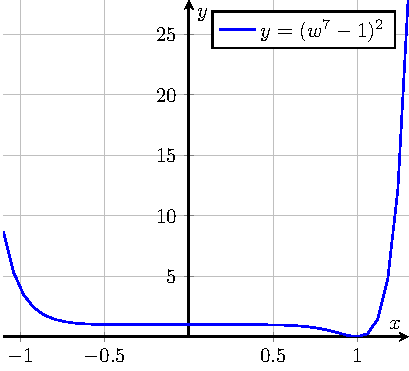
\includegraphics[height=0.42\textwidth]{First_lecture/figure_1.pdf}
\caption{Function Shape of $(w^7-1)^2$}
\label{Fig:2:1}
\end{figure}
\end{example}
From Figure~(\ref{Fig:2:1}) 
we can see that when $x\in[-0.5,0.5]$, the gradient of the loss function \emph{nearly} vanishes;
when $x>1.2$, the gradient exploses into infinite.
These two bad region makes the training~(optimization) process of such neural network very difficult.
\end{itemize}
\paragraph{How to rescue the gradient vanishing/explosion during DL training?}
The ``good'' region of the loss function is small. There are two ways to rescue this phenomenon:
\begin{enumerate}
\item
By proper initialization, it's possible to find a good region;
\item
By techniques such as \emph{Batch Normalization}, 
we can change the landscape of the loss function.
\end{enumerate}

\section{Back Propagation}
Suppose that the loss function is of finite-sum form:
\[
F(\theta)\triangleq\frac{1}{n}\sum_{i=1}^n\ell(f_\theta(x_i),y_i) 
\]
with 
$f_\theta(x_i) = W^L(\phi(W^{L-1}\phi(\cdots\phi(W(x)))))$, 
and the weight matrices $W^{\ell}$ are parameterized by $\theta$.
The direct motivation of \emph{back propagation} is to apply gradient descent
\footnote{Usually we use stochastic gradient descent method in DL since this method is more efficient} 
to minimize the loss function:
\[
\theta(t+1) = \theta(t) - \alpha_t\nabla F(\theta(t)).
\]
The non-trivial part during this process is how to tuning parameters $\alpha_t$ and how to compute 
$\nabla F(\theta(t))$.
The \emph{back propagation}~(BP) technique is one efficient strategy to compute the gradient by chain rule, since it avoids repeating the same computations.

\paragraph{Understanding BP in Level I: Scalar Form of Gradient}
Most courses/blogs teach how to do BP in scalar version, i.e., to compute the derivative of a scalar-valued function over a scalar variable, which are based on two rules:
\begin{itemize}
\item
Chain Rule: $f(g(w))$ with $f,g\in\mathbb{R}$,
\[
\frac{\diff f(g(w))}{\diff w} = \frac{\diff f}{\diff g}\frac{\diff g}{\diff w}
\]
\item
Sum rule: $g(w)\triangleq f_1(w)+f_2(w)$ with $w\in\mathbb{R}$,
\[
\frac{\diff g}{\diff w} = \frac{\diff f_1}{\diff w} + \frac{\diff f_2}{\diff w}
\]
\end{itemize}
We give an example on how to apply these two rules to compute the scalar form of the gradient of the loss function: 
\begin{example}
Consider a $2$-layer neural network with scalar output. We are interested in computing the derivative of this output $\hat{y}$ over a scalar parameter $w$.
%The model function can be represented as:
%\[
%\hat{y}(w) = 
%b\cdot(\phi(a\cdot\phi(w\cdot x_1))
%+
%d\cdot(\phi(c\cdot\phi(w\cdot x_1)) + M
%\]
%where $a,b,c,d,w$ are parameters to be chosen and $M$ is some constant independent of $w$.
This function w.r.t. $w$ can be represented in graph:
\begin{figure}[H]
\centering
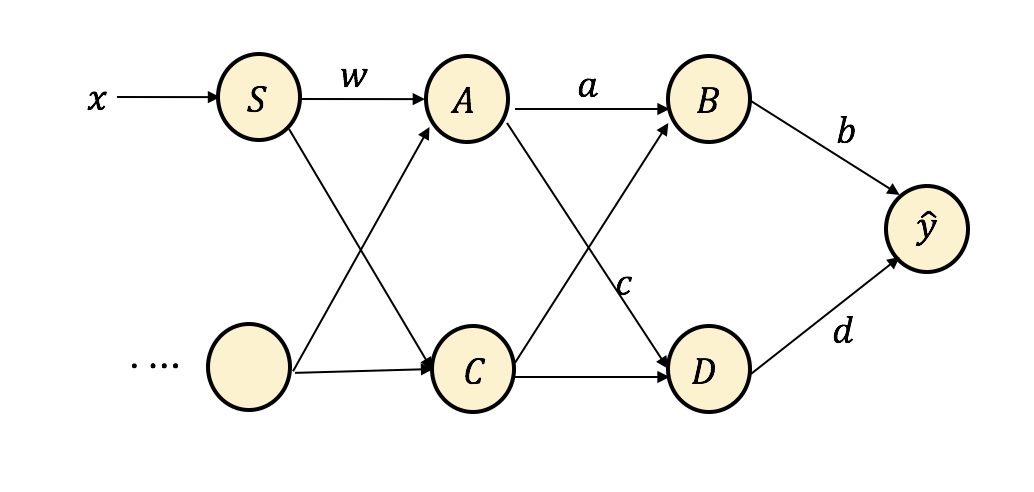
\includegraphics[width=0.9\textwidth]{Second_lecture/p_2}
\end{figure}
The computation of $\frac{\partial{\hat{y}}}{\partial{w}}$ can be summarized as follows:
\paragraph{Step 1: Decompose into multiple paths}
The path from the parameter $w$ to the output $\hat{y}$ undergoes two paths:
\[
\begin{array}{c}
w\to A\to B\to \hat{y}\\
w\to A\to D\to \hat{y}
\end{array}
\]
\paragraph{Step 2: Take gradient of each path by Chain rule}
These paths corresponds to the functions (w.r.t. $w$) as follows:
\begin{align*}
f_1(w)&=b\cdot\phi(a\cdot\phi(w\cdot x)\\
f_2(w)&=d\cdot\phi(c\cdot\phi(w\cdot x)
\end{align*}
The derivative of $f_1(w)$ is computed by the Chain rule:
\[
\frac{\partial f_1}{\partial w} = [b\cdot\phi'(a\cdot\phi(w\cdot x_1)]\cdot[a\cdot \phi'(w\cdot x)]\cdot [x]
\]
The derivative of $f_2(w)$ can be computed similarly.

\paragraph{Step 3: Take the sum of results from each path}
\end{example}
The coding is doable in this understanding level.

\paragraph{Understanding BP in Level II: Matrix Form of Gradient}
Firstly let's review some matrix calculus knowledge by an example.
\begin{example}
Consider a $2$-layer linear network\footnote{The weight matrices $U,V$ are parameterized by $\theta$} $f_{\theta}(x) = UVx.$ Given $n$ data points $(x_i,y_i)$, the goal is to minimize the loss function 
\[
F\triangleq\frac{1}{n}\sum_{i=1}^n\|UVx_i - y_i\|^2,
\]
with $U,V$ to be determined. The question is how to take gradient of $F$ w.r.t. the matrix $V$?
Or even simpler, how to compute $\frac{\partial F}{\partial V}$ with $F\triangleq\|UV-Y\|_F^2$? Here suppose that $U\in\mathbb{R}^{d_y\times d_1}$, $V\in\mathbb{R}^{d_1\times d_x}$, $Y\in\mathbb{R}^{d_y\times d_x}$.
\begin{itemize}
\item
Let's try to compute the gradient by ``standard'' Chain rule. Define $H=U\cdot V$, $E=H-Y$, and $F=\|E\|_F^2$.
\begin{align*}
\frac{\partial F}{\partial V}&=\frac{\partial F}{\partial E}\frac{\partial E}{\partial H}\frac{\partial H}{\partial V}\\
&=(2E)\cdot I\cdot(U)
\end{align*}
Then check the dimension. We find $E\in \mathbb{R}^{d_y\times d_x}$ and $U\in \mathbb{R}^{d_y\times d_1}$. The matrix-multiplication is undefined!
If we want to make the dimension matched, we should write
\[
\frac{\partial F}{\partial V} = 2U\trans E.
\]
\end{itemize}
Sometimes it's problematic to write gradient by checking matrix dimensions. For instance, if $d_y=d_x$ in practice, this method is invalid.
Another way is to write down scalar-input scalar-output derivatives and then form the whole matrix\footnote{LeCun, CS224 Note, \url{https://web.stanford.edu/class/cs224n/}}. However, this way is tedious in practice. 

The reason why our method is problematic is that we probably applied the Chain rule incorrectly. 
Wikipedia provides the Chain rule for vector-valued functions:
\begin{proposition}[Vector-Function Chain Rule]\label{pro:2:1}
For vector-input vector-output functions
\[
x\in\mathbb{R}^{n}\to g(x)\in\mathbb{R}^m\to F(x)\triangleq f(g(x))\in\mathbb{R}^k,
\]
%\[
%I(X;Y\mid Z=z) = I(X\mid Z=z;Y\mid Z=z)
%\]
the chain rule is
\[
\frac{\partial F}{\partial x} = \frac{\partial f(g(x))}{\partial g(x)}\frac{\partial g(x)}{\partial x},
\]
where
\[
\frac{\partial f(g(x))}{\partial x}= \left[\frac{\partial f_i(g(x_j))}{\partial x_j}\right]_{ij}\in\mathbb{R}^{k\times m},\quad
\frac{\partial g(x)}{\partial x} = \left[\frac{\partial g_i}{\partial x_j}\right]_{ij}\in\mathbb{R}^{m\times n}
\]
denotes the Jacobian matrices.
\end{proposition}
\begin{itemize}
\item
Consider the objective function $F= \|UV x - y\|_F^2.$
The goal is to apply proposition~(\ref{pro:2:1}) to write $\frac{\partial F}{\partial V}$. 
\begin{figure}[H]
\centering
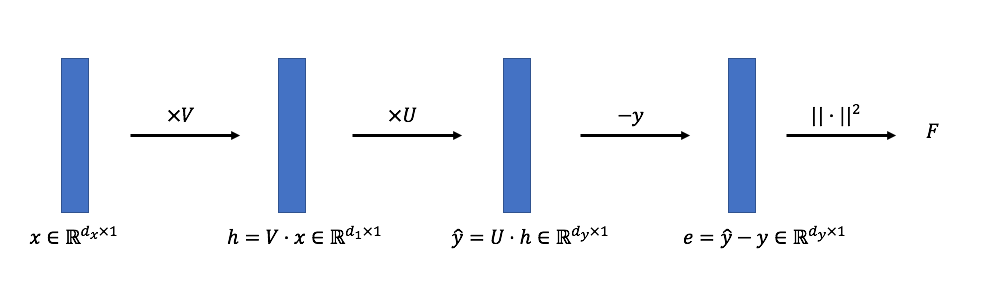
\includegraphics[width=\textwidth]{Second_lecture/p_3}
\caption{Diagram for the operator $F$}
\end{figure}
As a result,
\[
\frac{\partial F}{\partial V} = \frac{\partial F}{\partial e}\frac{\partial e}{\partial\hat{y}}\frac{\partial\hat{y}}{\partial h}\frac{\partial h}{\partial V}
\]
In this formula, the LHS is of the form ($\partial$ scalar/$\partial$ matrix), which should be a matrix;
the first term in RHS is of the form ($\partial$ scalar/$\partial$ vector), which should be a vector; the second and third term in RHS are of the form ($\partial$ vector/$\partial$ vector), which should be a matrix; the forth term is of the form ($\partial$ vector/$\partial$ matrix), which should be a tensor. 
Here we discuss the issues for computing these derivatives:
\begin{enumerate}
\item
Issue 1: computing derivative of a scalar over a vector.

The issue for computing $\frac{\partial F}{\partial e}$ is on the confusion of the different notions of derivatives.
\begin{itemize}
\item
By definition of Jacobian matrices from proposition~(\ref{pro:2:1}), $\frac{\partial F}{\partial e}\in\mathbb{R}^{\text{fan-out}\times\text{fan-in}}=\mathbb{R}^{1\times d_y}$, which is a row vector;
\item
By definition of gradient, we assume $\frac{\partial F}{\partial e}$ is a column vector instead, i.e., a vector of dimension $d_y\times 1$.
\item
Moreover, the notion of Jacobian and gradient coincides\footnote{At least in some references, e.g., Matrix Differentiation, available at \url{https://atmos.washington.edu/~dennis/MatrixCalculus.pdf}} for the case $\text{fan-out}>1$, e.g.,
\[
\frac{\partial(Wx)}{\partial x}=W.
\]
\end{itemize}
Based on the issues above, one solution is to define the \emph{general Jacobian} to unify the notions of gradient and Jacobian. Before that, from now on, we define $\frac{{\partial} f}{{\partial} x}$ as a row vector if $f$ is scalar-valued, otherwise $\frac{{\partial} f}{{\partial} x}$ denotes the Jacobian matrix. Moreover, define the \emph{general Jacobian} 
\[
\frac{\tilde{\partial} f}{\tilde{\partial} x}=\left\{
\begin{aligned}
\frac{\partial f}{\partial x},&\quad\text{if fan-out$>1$ and fan-in$>1$}\\
\left(\frac{\partial f}{\partial x}\right)\trans,&\quad\text{if fan-out $=1$}
\end{aligned}
\right.
\]
\emph{The proposition~(\ref{pro:2:1})} always holds for \emph{general Jacobian}. Intermediately,
\[
\frac{\tilde{\partial} F}{\tilde{\partial} h} =
\frac{\tilde{\partial} F}{\tilde{\partial} e} 
\frac{\tilde{\partial} e}{\tilde{\partial} h} 
\implies
\left(\frac{\tilde{\partial} F}{\tilde{\partial} h}\right)\trans =
\left(\frac{\tilde{\partial} e}{\tilde{\partial} h} \right)\trans
\left(\frac{\tilde{\partial} F}{\tilde{\partial} e}\right)\trans
\]
Or equivalently,
\begin{equation}\label{Eq:2:1}
\begin{array}{lcll}
\frac{{\partial} F}{{\partial} h}
&
=
&
\left(\frac{{\partial} e}{{\partial} h} \right)\trans
&
\left(\frac{{\partial} F}{{\partial} e}\right)\\
~\uparrow&&\quad\uparrow&\quad\uparrow\\
\frac{\partial\text{ scalar}}{\partial\text{ vector}}
&
&
\frac{\partial\text{ vector}}{\partial\text{ vector}}
&
\frac{\partial\text{ scalar}}{\partial\text{ vector}}
\end{array}
\end{equation}
\item
Issue 2: computing derivative of a vector over a matrix.

There are two ways to solve this issue:
\begin{itemize}
\item
The first way is to reduce matrix into vectors, i.e., in order  to compute $\frac{\partial F}{\partial V}$, it suffices to consider $\frac{\partial F}{\partial V(:,k)}$ and then combine to form a tensor.
\item
The other is to use Lemma~(\ref{lemma:2:1}) that deals vector-matrix derivative into the vector-vector cases.
\end{itemize}
Let's consider the second way in this lecture.
\begin{lemma}\label{lemma:2:1}
For $g(V)\triangleq\phi(Vx)$ with $x\in\mathbb{R}^{d\times 1}$ and $V\in\mathbb{R}^{k\times d}$, define $h=Vx$. Then
\[
\frac{\partial g}{\partial V} = \frac{\partial\phi}{\partial h}x\trans
\]
\end{lemma}
Now we give an example for applying Lemma~(\ref{lemma:2:1}) to compute $\frac{\partial F}{\partial V}$:
\begin{subequations}
\begin{align}
\frac{\partial F}{\partial V} &= \frac{\partial F}{\partial h}x\trans\label{Eq:2:2a}\\
&=\left(\frac{{\partial} e}{{\partial} h} \right)\trans\left(\frac{{\partial} F}{{\partial} e}\right)x\trans\label{Eq:2:2b}\\
&=\left(\frac{{\partial} e}{{\partial} \hat{y}}\frac{{\partial}\hat{y}}{{\partial}h} \right)\trans\left(\frac{{\partial} F}{{\partial} e}\right)x\trans\label{Eq:2:2c}\\
&=(I\cdot U)\trans 2e\cdot x\trans\label{Eq:2:2d}\\
&=2U\trans ex\trans\nonumber
\end{align}
\end{subequations}
where (\ref{Eq:2:2a}) is because of Lemma~(\ref{lemma:2:1}) and $F(V)=F(Vx)$;
(\ref{Eq:2:2b}) is by the substitution of (\ref{Eq:2:1});
(\ref{Eq:2:2c}) is by the Chain rule stated in proposition~(\ref{pro:2:1});
(\ref{Eq:2:2d}) is by direct calculation.
\end{enumerate}
Exercise: 
\[
\frac{\partial \|AWB + C\|_F^2}{\partial W} = 2A\trans(AWB+C)B\trans
\]
\end{itemize}
\end{example}


\paragraph{BP for General Deep Non-linear Network}
Now derive the gradient of fully-connected neural network with quadratic loss. 
The objective $f_\theta$ is defined based on the following diagram:
\begin{figure}[H]
\centering

\includegraphics[width=\textwidth]{Second_lecture/p_4}
\caption{Diagram for the operator $F$}
\end{figure}
Then the derivative $\frac{\partial F}{\partial W^1}$ is computed as follows:
\begin{subequations}
\begin{align}
\frac{\partial F}{\partial W^1} &= \frac{\partial F}{\partial h^1}x\trans\label{Eq:2:3a}\\
&=\left(\frac{\partial e}{\partial h^1}\right)\trans\left(\frac{\partial F}{\partial e}\right)x\trans\label{Eq:2:3b}\\
&=\left(\frac{\partial e}{\partial h^1}\right)\trans 2e\cdot x\trans\nonumber\\
&=\left(
\frac{\partial e}{\partial h^L}\frac{\partial h^L}{\partial z^{L-1}}\cdots\frac{\partial h^1}{\partial z^1}\frac{\partial z^1}{\partial h^1}
\right)\trans2e\cdot x\trans\label{Eq:2:3d}\\
&=\bigg(W^LD^{L-1}W^{L-1}D^{L-2}\cdots W^2D^1\bigg)\trans2e\cdot x\trans\label{Eq:2:3e}
\end{align}
\end{subequations}
where (\ref{Eq:2:3a}) is by Lemma~(\ref{lemma:2:1});
(\ref{Eq:2:3b}) follows the similar trick as in (\ref{Eq:2:1});
(\ref{Eq:2:3d}) is by the Chain rule stated in proposition~(\ref{pro:2:1});
in (\ref{Eq:2:3e}) the matrix $D^{\ell}\triangleq\diag(\phi'(h_i^{\ell}))_{i=1}^{d_{\ell}}$, with $\phi'$ denotes the derivative of $\phi$.
The general formula $\frac{\partial F}{\partial W^{\ell}}$ is left as exercise: 
\[
\frac{\partial F}{\partial W^{\ell}}=
(W^{L}D^{L-1}\cdots W^{\ell+1}D^{\ell})\trans\cdot 2e\cdot(z^{\ell-1})\trans
\]
This formula can be expressed in a recursive way, which is the mechanism of the BP technique.  
BP is an efficient way to compute all gradients $\frac{\partial F}{\partial W^{\ell}}$ for $\ell=1,\dots,L$.
The navie computation complexity is $\mathcal{O}(d^2L^2)$; while the BP complexity is $\mathcal{O}(d^2L)$.


\section{Initialization methods for handling Training Difficulty}\label{sec:2:3}
We have discussed the \emph{gradient explosion or vanishing} issue. The step size for the gradient descent method is one over the Lipschitz constant, which will be super-small/super-large in gradient explosion/vanishing cases. From the landscape in Fig.~(\ref{Fig:2:1}), we can see that $w^7$ grows more active compared with the input $x=1$. 
To solve this problem, the direct idea is to control the ``energy'' of output compared with the input, i.e., for linear network $y=W^LW^{L-1}\cdots W^1\cdot x$,
we want to have
\[
\|W^LW^{L-1}\cdots W^1\cdot x\|\approx\|x\|.
\]
Or even simpler, maybe it's enough to let $\|W^{\ell}x\|\approx\|x\|$ for $\ell=1,\dots,L$.
Assume $W^{\ell}$ is initialized to be a random matrix.
After simulation we found that the energy~($\ell_2$ norm) for the output after activation is much larger than the previous input.
\begin{verbatim}
clear;
d = 100;		% dimension for weight matrix W
maxit = 10;	% maximum iteration number	

x = ones(d,1);  norm0 = norm(x);
for i = 1:maxit
    W = randn(d,d);
    x = W*x;
    rato = norm(x)/norm0
end
\end{verbatim}
There are different ways to deal with this problem:
\begin{itemize}
\item
Sparsity Solution: Set many entries of $W$ to be $0$;
\item
Orthogonalization: Generate orthogonal random weight matrix; (to be discussed in the future)
\item
Scalization: Normalize each entry of $W$ by some constant $C$.
\end{itemize}
We find that if each entry of $W$~(assume to be square matrix first) is divided by $\sqrt{d}$, then the energy of $\|W\cdot x\|$ is very close to $\|x\|$.

\begin{quotation}
Informal Xavier Initialization:
for the special case where $d=d_x=d_1=\cdots=d_{L-1}=d_L$, initialize
\begin{equation*}
W^{\ell}_{i,j}\sim\mathcal{N}(0,1)\cdot\frac{1}{\sqrt{d}}
\end{equation*}
\end{quotation}
\paragraph{Supporting Analysis}
\begin{enumerate}
\item
Claim 1: For fixed $x$, if entries of $W$ are i.i.d. such that 
\begin{equation}\label{Eq:2:4}
W_{i,j}\sim\mathcal{N}(0,1/d),\footnote{for the case $\text{fan-in}\ne\text{fan-out}$, use $W_{i,j}\sim\mathcal{N}(0,1/d_{\text{fan-out}})$}
\end{equation}
then 
\[
\mathbb{E}\|Wx\|^2 = \|x\|^2.
\]
\begin{proof}
Two-line proof: $\mathbb{E}\|Wx\|^2=x\trans \mathbb{E}[W\trans W]x$ and
evaluate the term $\mathbb{E}[W\trans W]$.
\end{proof}
Sometimes $x$ are also initialized as random number. Therefore, there is a stronger version of claim 1.
\item
Claim 2: if $x_i$'s are i.i.d., and previous conditon holds\footnote{Again, for the case $\text{fan-in}\ne\text{fan-out}$, follow the setting in claim 1.}, and $x$ is independent of $W$, then 
\[
\mathbb{E}\|Wx\|^2 = \|x\|^2.
\]
\end{enumerate}

\begin{remark}
\begin{enumerate}
\item
If the input and the output dimension are not the same, there is an in-consistency in (\ref{Eq:2:4}). In this case, we try $W_{i,j}^{\ell}\sim\mathcal{N}(0,2/(d_{\text{fan-in}}+d_{\text{fan-out}}))$.
This is the formal Xavier Initialization.
\item
The claims 1 and 2 are only about feed-forward neural network.
For the back-ward case, i.e., $e^1 = (W^LW^{L-1}\cdots W^1)\trans e$, 
we need to have $W_{ij}\sim\mathcal{N}(0,1/d_{\text{fan-in}})$.
\item
The conditions for claims 1 and 2 can be weakened a little bit, e.g., the Gaussian assumptions of $W$ are not needed but only the mean and variance assumptions.
\item
For non-linear activation such as relu function, the He Initialization / Kaming Initialization is needed. The initution is that $\mathbb{E}[\text{Relu}(w^2)]=1/2$. In this case, initialize
\[
\mathbb{E}W_{ij}^{\ell} = 0,\quad
\text{Var}(W_{ij}^{\ell}) =\frac{2}{\text{fan-in}}\quad\text{or}\frac{2}{\text{fan-out}}
\]
\end{enumerate}
\end{remark}










